\documentclass{article}
\usepackage[margin=1in]{geometry}
\usepackage{amsmath}
\usepackage{amssymb}
\usepackage{amsthm}
\usepackage{bm}
\usepackage{hyperref}
\usepackage{graphicx}
\usepackage{caption}
\usepackage{listings}
\usepackage{xcolor}
\usepackage{float}
\usepackage{placeins}
\graphicspath{{figures/}}

% Code style
\lstdefinestyle{code}{
  basicstyle=\ttfamily\small,
  numbers=left,
  numberstyle=\tiny,
  numbersep=8pt,
  keywordstyle=\color{blue},
  commentstyle=\color{teal!70!black},
  stringstyle=\color{orange!70!black},
  showstringspaces=false,
  breaklines=true,
  frame=single,
  framerule=0.3pt,
  rulecolor=\color{black!15}
}
\lstset{style=code}

\title{Graph Neural Networks: Spectral Foundations and Real-World Applications}
\author{}
\date{\today}

\begin{document}
\maketitle
\tableofcontents
\FloatBarrier

\section{Graph Convolutional Networks (GCN)}
Graph convolutional networks generalize convolution to irregular graph domains. For an undirected graph $G = (\mathcal{V}, \mathcal{E})$ with adjacency matrix $\mathbf{A}$ and node features $\mathbf{X} \in \mathbb{R}^{|\mathcal{V}| \times d}$, spectral graph theory provides the foundation for filtering operations. Figure~\ref{fig:gcn_graph_structure} highlights the neighborhood aggregation process.

\subsection{Spectral Formulation}
Let $\mathbf{L} = \mathbf{D} - \mathbf{A}$ denote the combinatorial Laplacian with degree matrix $\mathbf{D}$. The eigendecomposition $\mathbf{L} = \mathbf{U} \boldsymbol{\Lambda} \mathbf{U}^\top$ yields graph Fourier bases. A spectral filter $g_\theta(\boldsymbol{\Lambda})$ applied to signal $\mathbf{X}$ is
\begin{equation}
  g_\theta \star \mathbf{X} = \mathbf{U} g_\theta(\boldsymbol{\Lambda}) \mathbf{U}^\top \mathbf{X}.
\end{equation}
Chebyshev polynomials approximate $g_\theta$ with $K$-hop support:
\begin{equation}
  g_\theta \star \mathbf{X} \approx \sum_{k=0}^{K} \theta_k T_k(\tilde{\mathbf{L}}) \mathbf{X}, \quad \tilde{\mathbf{L}} = \frac{2}{\lambda_{\max}} \mathbf{L} - \mathbf{I},
\end{equation}
where $T_k$ is the Chebyshev polynomial of order $k$. Kipf and Welling simplify to first-order ($K=1$) by constraining $\theta$:
\begin{equation}
  \mathbf{H}^{(l+1)} = \sigma\left(\tilde{\mathbf{D}}^{-1/2} \tilde{\mathbf{A}} \tilde{\mathbf{D}}^{-1/2} \mathbf{H}^{(l)} \mathbf{W}^{(l)}\right),
\end{equation}
with $\tilde{\mathbf{A}} = \mathbf{A} + \mathbf{I}$ and $\tilde{\mathbf{D}}_{ii} = \sum_j \tilde{\mathbf{A}}_{ij}$. This renormalization ensures numerical stability by symmetrically normalizing self-loops.

\subsection{Message Passing Interpretation}
The GCN layer can be viewed as message passing where nodes update via averaged neighbor features:
\begin{equation}
  \mathbf{h}_v^{(l+1)} = \sigma\left(\sum_{u \in \mathcal{N}(v) \cup \{v\}} \frac{1}{\sqrt{\tilde{d}_v \tilde{d}_u}} \mathbf{h}_u^{(l)} \mathbf{W}^{(l)}\right),
\end{equation}
where $\tilde{d}_v$ counts neighbors with self-loop. Figure~\ref{fig:gcn_layer_flow} depicts the flow of information across two GCN layers.

\subsection{Over-smoothing and Remedies}
Stacking many GCN layers causes node embeddings to converge, a phenomenon known as over-smoothing. Mitigation strategies include residual/skip connections, normalization (PairNorm, BatchNorm), and personalized propagation (APPNP) that blends teleportation:
\begin{equation}
  \mathbf{Z} = (1-\alpha) \left(\mathbf{I} - \alpha \tilde{\mathbf{P}}\right)^{-1} \mathbf{H}^{(K)},
\end{equation}
with $\tilde{\mathbf{P}} = \tilde{\mathbf{D}}^{-1} \tilde{\mathbf{A}}$.

\subsection{Training Pipeline}
\begin{lstlisting}[language=Python, caption={Two-layer GCN for semi-supervised node classification (PyTorch Geometric).}]
import torch
import torch.nn.functional as F
from torch_geometric.nn import GCNConv

class GCN(torch.nn.Module):
    def __init__(self, in_dim, hidden_dim, out_dim, dropout=0.5):
        super().__init__()
        self.conv1 = GCNConv(in_dim, hidden_dim, normalize=True)
        self.conv2 = GCNConv(hidden_dim, out_dim, normalize=True)
        self.dropout = dropout

    def forward(self, x, edge_index):
        x = self.conv1(x, edge_index)
        x = F.relu(x)
        x = F.dropout(x, p=self.dropout, training=self.training)
        x = self.conv2(x, edge_index)
        return F.log_softmax(x, dim=1)

model = GCN(dataset.num_node_features, 64, dataset.num_classes)
optimizer = torch.optim.Adam(model.parameters(), lr=0.01, weight_decay=5e-4)

for epoch in range(200):
    model.train()
    optimizer.zero_grad()
    out = model(data.x, data.edge_index)
    loss = F.nll_loss(out[data.train_mask], data.y[data.train_mask])
    loss.backward()
    optimizer.step()
\end{lstlisting}

\begin{figure}[H]
  \centering
  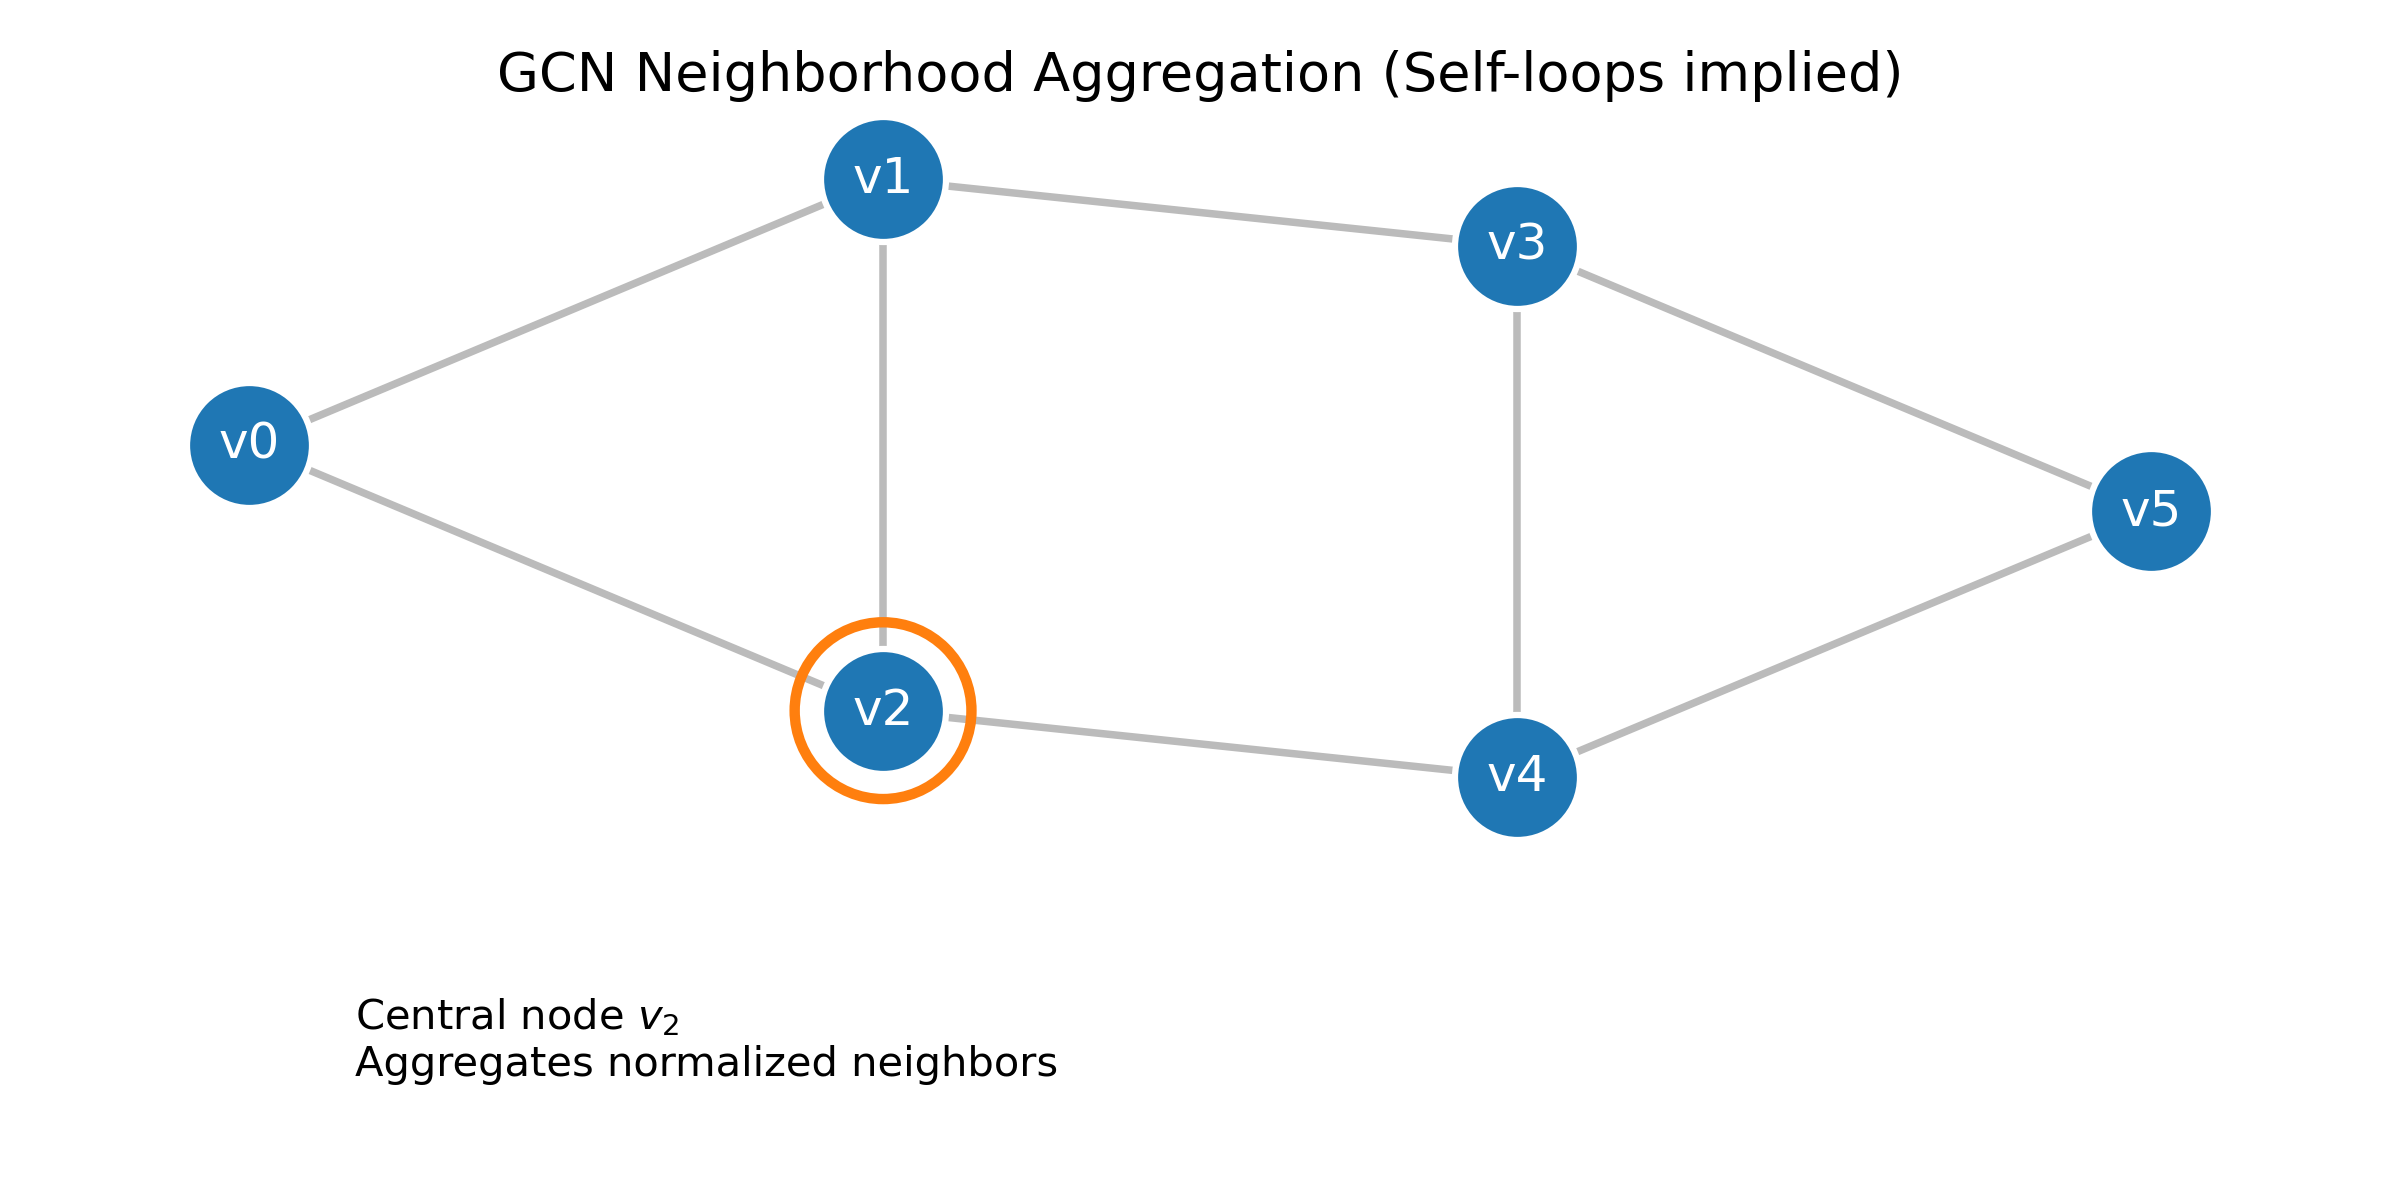
\includegraphics[width=0.75\textwidth]{gcn_graph_structure.png}
  \caption{Graph convolution aggregates normalized neighbor information including self-loops. Degree normalization controls scale.}
  \label{fig:gcn_graph_structure}
\end{figure}

\begin{figure}[H]
  \centering
  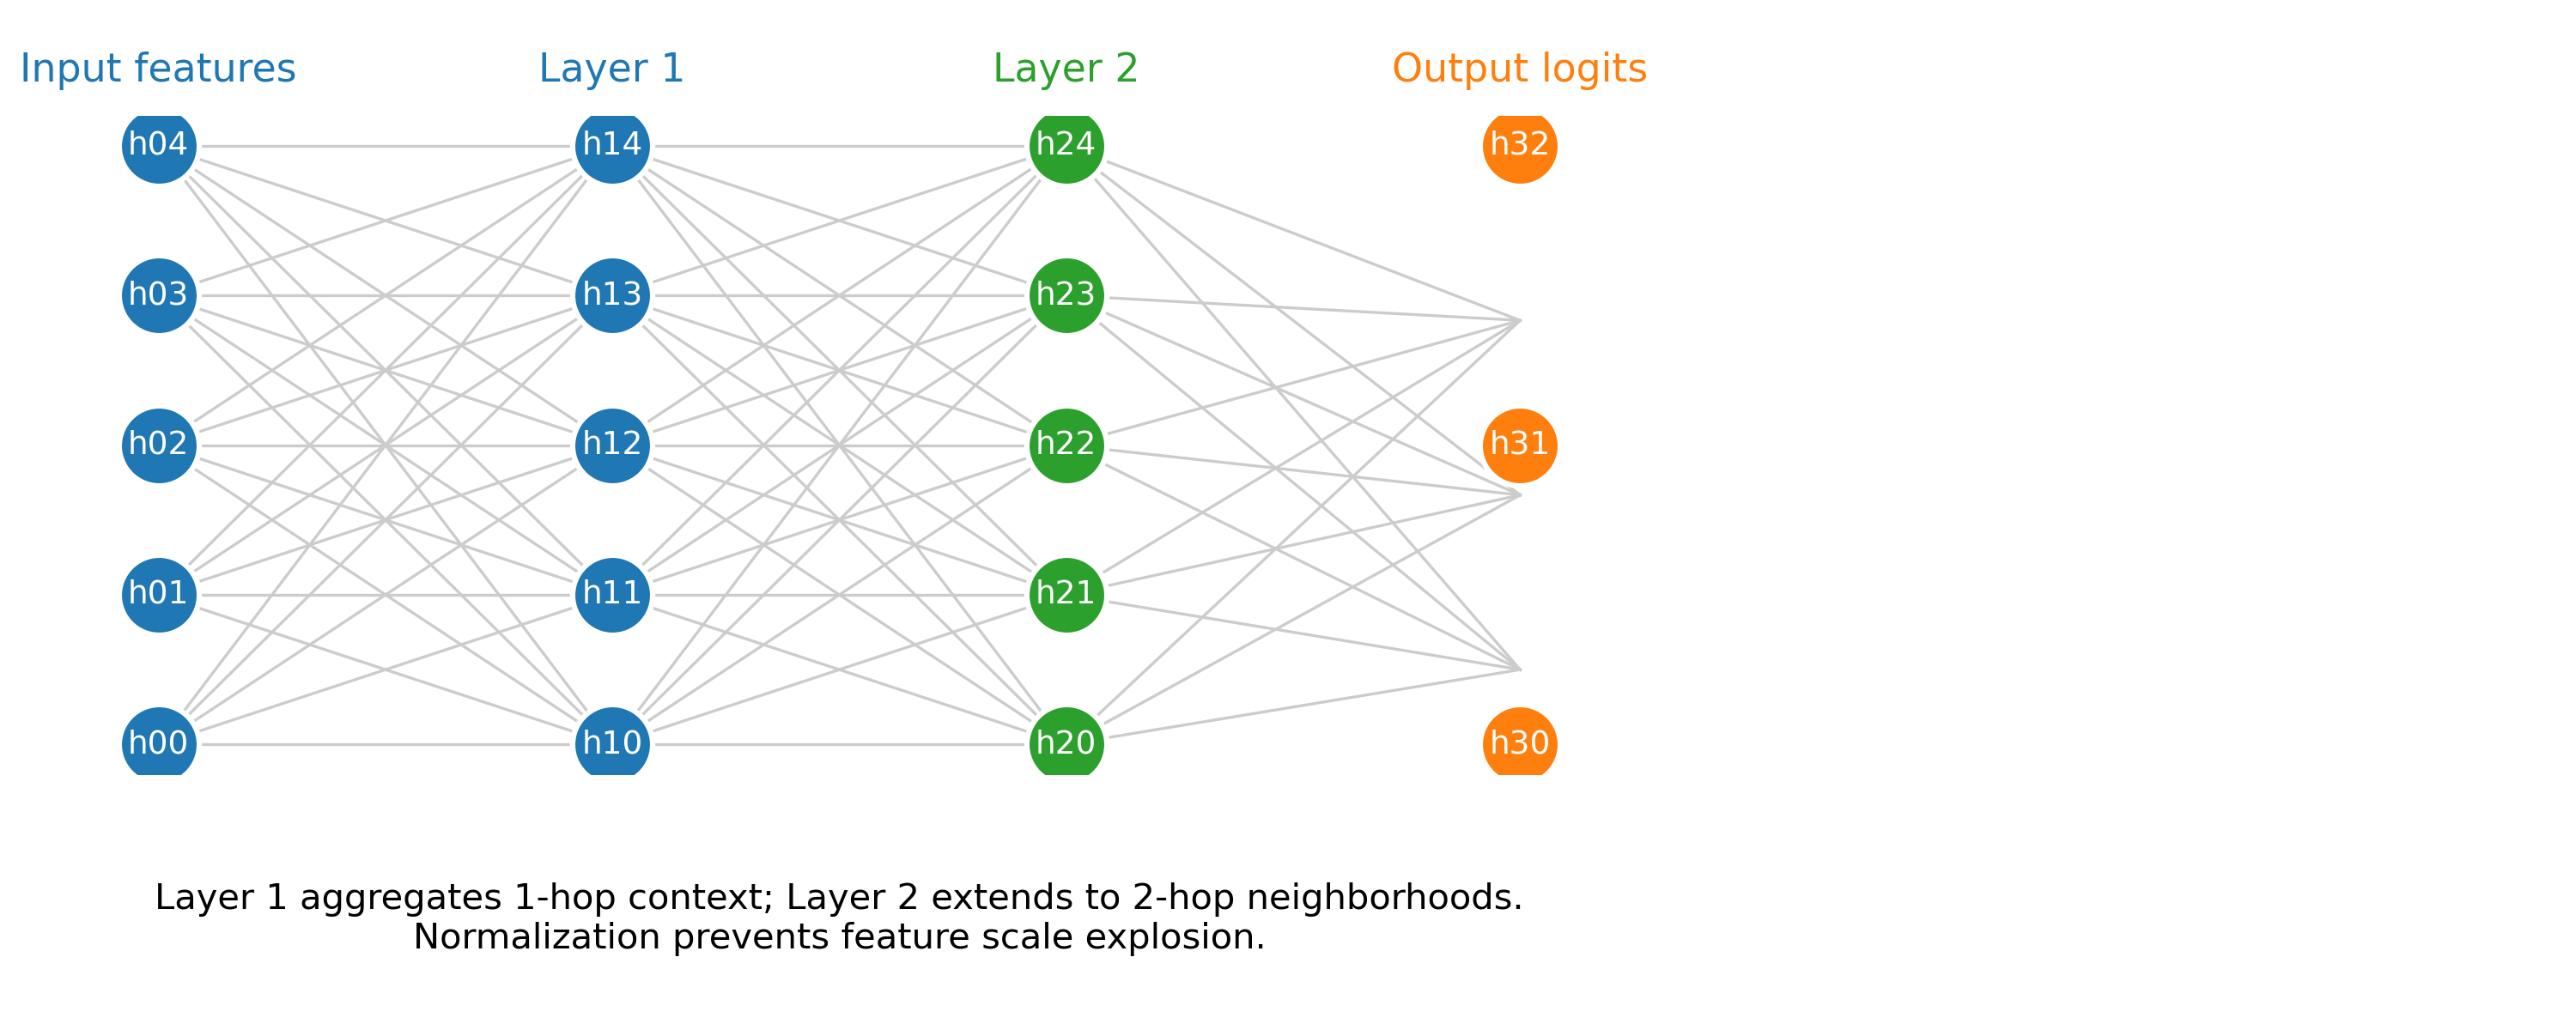
\includegraphics[width=0.85\textwidth]{gcn_layer_flow.png}
  \caption{Two-layer GCN message passing: layer 1 captures one-hop neighborhoods, layer 2 extends to two hops.}
  \label{fig:gcn_layer_flow}
\end{figure}
\FloatBarrier

\section{Applications: Social Networks, Molecular Prediction, Recommender Systems}
GCNs and related GNN architectures excel in domains where relational inductive biases matter. Figure~\ref{fig:gnn_application_landscape} sketches representative pipelines.

\subsection{Social Network Analysis}
In social graphs, GCNs embed users with homophily-aware features. Tasks include community detection, influence prediction, and content recommendation. Heterogeneous graphs (users, posts, tags) demand relational GCN (R-GCN) with relation-specific weight matrices:
\begin{equation}
  \mathbf{h}_v^{(l+1)} = \sigma \left( \sum_{r \in \mathcal{R}} \sum_{u \in \mathcal{N}_r(v)} \frac{1}{c_{v,r}} \mathbf{W}_r^{(l)} \mathbf{h}_u^{(l)} + \mathbf{W}_0^{(l)} \mathbf{h}_v^{(l)} \right).
\end{equation}
Graph sampling strategies (GraphSAGE, Cluster-GCN) support billion-edge training by subsampling neighborhoods.

\subsection{Molecular Property Prediction}
Molecules map naturally to graphs with atoms as nodes and bonds as edges. Message passing neural networks (MPNNs) generalize GCNs with edge updates:
\begin{align}
  \mathbf{m}_v^{(l+1)} &= \sum_{u \in \mathcal{N}(v)} \phi^{(l)}\left(\mathbf{h}_v^{(l)}, \mathbf{h}_u^{(l)}, \mathbf{e}_{uv}\right), \\
  \mathbf{h}_v^{(l+1)} &= \psi^{(l)}\left(\mathbf{h}_v^{(l)}, \mathbf{m}_v^{(l+1)}\right),
\end{align}
where $\mathbf{e}_{uv}$ encodes bond types. Global pooling ($\sum$, mean, set2set) aggregates molecular fingerprints. Combining quantum-inspired features and equivariant architectures (E(n)-GNN) yields state-of-the-art performance on QM9 and Materials Project benchmarks.

\subsection{Recommender Systems}
User-item interactions form bipartite graphs. LightGCN simplifies GCNs by removing nonlinearities and feature transformations:
\begin{equation}
  \mathbf{E}^{(k+1)} = \tilde{\mathbf{D}}^{-1/2} \tilde{\mathbf{A}} \tilde{\mathbf{D}}^{-1/2} \mathbf{E}^{(k)}, \qquad \mathbf{E} = \frac{1}{K+1} \sum_{k=0}^{K} \mathbf{E}^{(k)}.
\end{equation}
The final embeddings produce recommendation scores via inner products, $s_{ui} = \mathbf{e}_u^\top \mathbf{e}_i$. Real-world systems incorporate temporal dynamics, side information, and counterfactual debiasing.

\subsection{Deployment Considerations}
\begin{itemize}
  \item \textbf{Scalability:} Neighbor sampling (PinSAGE), graph partitioning, and multi-GPU training handle web-scale graphs.
  \item \textbf{Explainability:} GNNExplainer and GraphMask identify influential substructures for decision transparency.
  \item \textbf{Robustness:} Adversarial perturbations on edges/nodes degrade performance; defense strategies include adversarial training and certified robustness via randomized smoothing.
\end{itemize}

\begin{figure}[H]
  \centering
  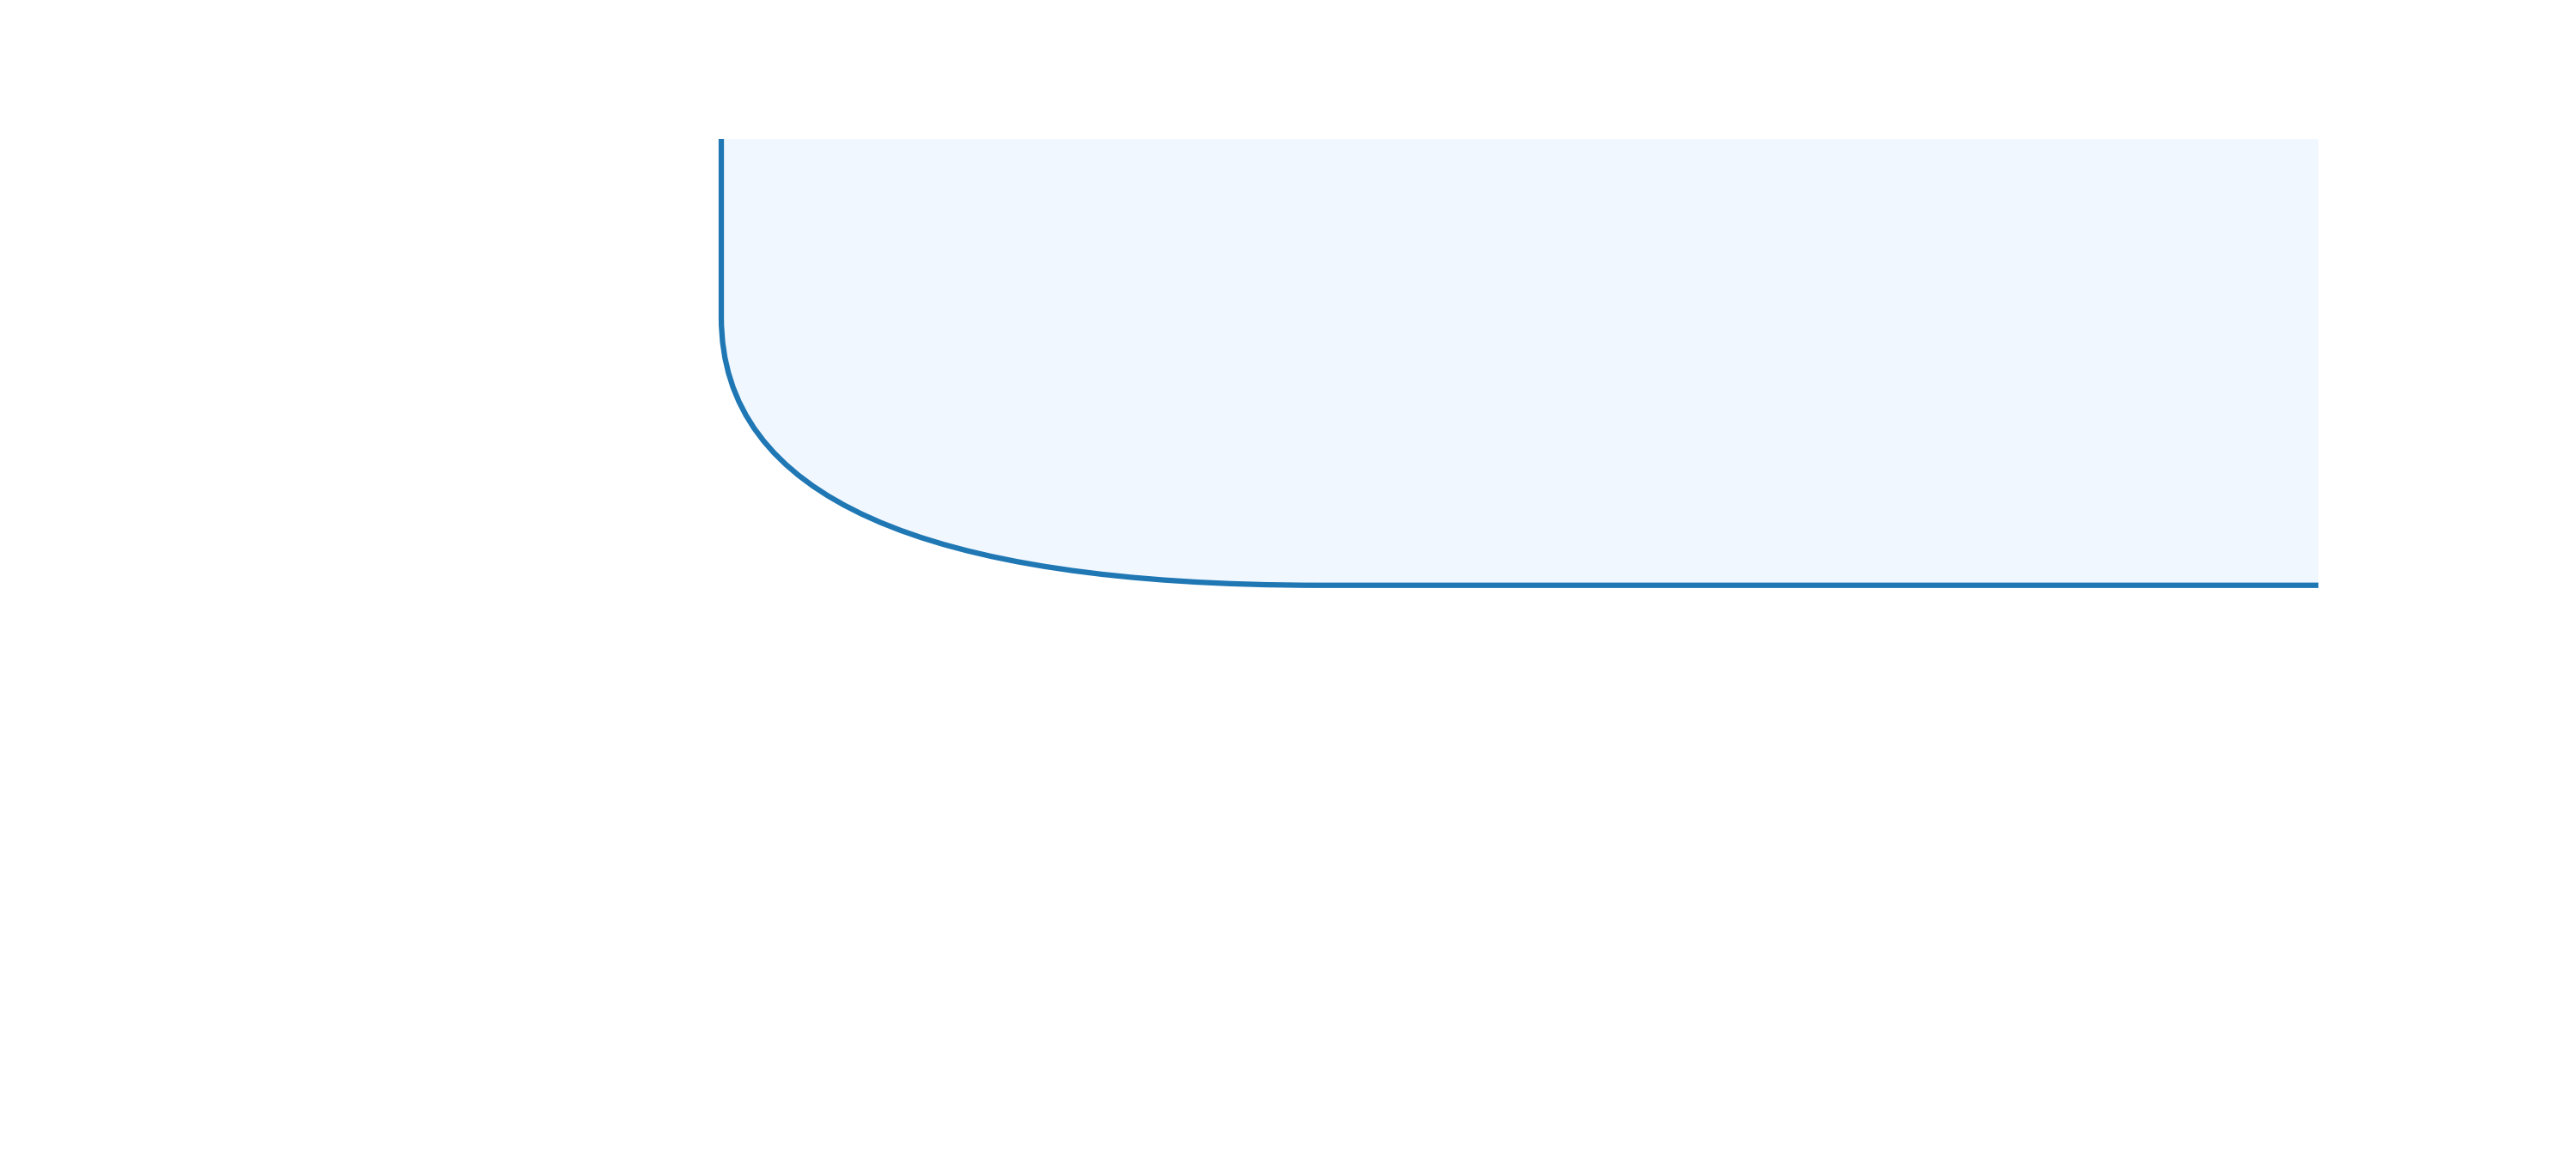
\includegraphics[width=0.9\textwidth]{gnn_application_landscape.png}
  \caption{Applications of GNNs across social graphs, molecular chemistry, and recommender systems with domain-specific modules.}
  \label{fig:gnn_application_landscape}
\end{figure}
\FloatBarrier

\section*{Further Reading}
\begin{itemize}
  \item Thomas N. Kipf and Max Welling. ``Semi-Supervised Classification with Graph Convolutional Networks.'' ICLR 2017.
  \item Petar Veličković et al. ``Graph Attention Networks.'' ICLR 2018.
  \item Will Hamilton et al. ``Inductive Representation Learning on Large Graphs.'' NIPS 2017.
  \item Keyulu Xu et al. ``How Powerful are Graph Neural Networks?'' ICLR 2019.
  \item He et al. ``LightGCN: Simplifying and Powering Graph Convolution Network for Recommendation.'' SIGIR 2020.
\end{itemize}

\end{document}
